

\begin{frame}
	\frametitle{Example}

    Colour one side of the future cut red and the other blue.
	\center
	\begin{multicols}{2}

        Input graph (spanning tree thick) \\
	\medskip
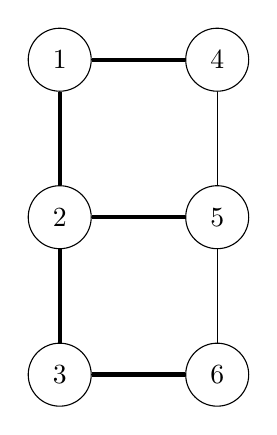
\begin{tikzpicture}[
  vertex/.style={draw,circle,minimum size=0.8cm},
  every node/.style={vertex},
  spanning_tree/.style={draw=black, ultra thick}
  ]
	\node (1) at (1,5) {1};
	\node (2) at (1,3) {2};
	\node (3) at (1,1) {3};

	\node (4) at (3,5) {4};
	\node (5) at (3,3) {5};
	\node (6) at (3,1) {6};

	\draw[spanning_tree] (1) -- (2);
	\draw[spanning_tree] (2) -- (3);

	\draw (4) -- (5);
	\draw (5) -- (6);

	\draw[spanning_tree] (1) -- (4);
	\draw[spanning_tree] (2) -- (5);
	\draw[spanning_tree] (3) -- (6);
\end{tikzpicture}
\\
$   $ \\

1. step \\
	\medskip
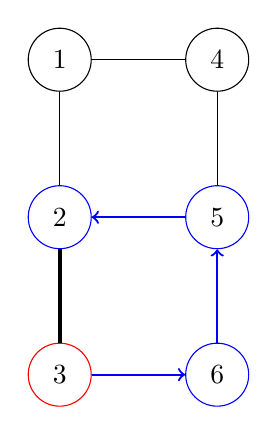
\begin{tikzpicture}[
  vertex/.style={draw,circle,minimum size=0.8cm},
  every node/.style={vertex},
  red_vertex/.style={draw=red},
  blue_vertex/.style={draw=blue},
  inx/.style={draw=black, ultra thick},
  onc/.style={draw=blue, thick}
  ]
	\node (1) at (1,5) {1};
	\node[blue_vertex] (2) at (1,3) {2};
	\node[red_vertex] (3) at (1,1) {3};

	\node (4) at (3,5) {4};
	\node[blue_vertex] (5) at (3,3) {5};
	\node[blue_vertex] (6) at (3,1) {6};

	\draw (1) -- (2);
	\draw[inx] (2) -- (3);

	\draw (4) -- (5);
	\draw[onc,<-] (5) -- (6);

	\draw (1) -- (4);
	\draw[onc, <-] (2) -- (5);
	\draw[onc, ->] (3) -- (6);
\end{tikzpicture}
 \\
 $X = \{ (2,3) \}$
	\end{multicols}

\end{frame}


\begin{frame}
	\frametitle{Example}

    Colour one side of the future cut red and the other blue.

	\center
	\begin{multicols}{2}

1. step \\
	\medskip
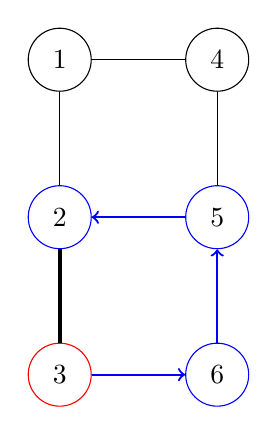
\begin{tikzpicture}[
  vertex/.style={draw,circle,minimum size=0.8cm},
  every node/.style={vertex},
  red_vertex/.style={draw=red},
  blue_vertex/.style={draw=blue},
  inx/.style={draw=black, ultra thick},
  red_edge/.style={draw=red, ultra thick},
  onc/.style={draw=blue, thick}
  ]
	\node (1) at (1,5) {1};
	\node[blue_vertex] (2) at (1,3) {2};
	\node[red_vertex] (3) at (1,1) {3};

	\node (4) at (3,5) {4};
	\node[blue_vertex] (5) at (3,3) {5};
	\node[blue_vertex] (6) at (3,1) {6};

	\draw (1) -- (2);
	\draw[inx] (2) -- (3);

	\draw (4) -- (5);
	\draw[onc, <-] (5) -- (6);

	\draw (1) -- (4);
	\draw[onc, <-] (2) -- (5);
	\draw[onc,->] (3) -- (6);
\end{tikzpicture}
 \\
 $X = \{ (2,3) \}$

1. step, 1. recursive call \\
	\medskip
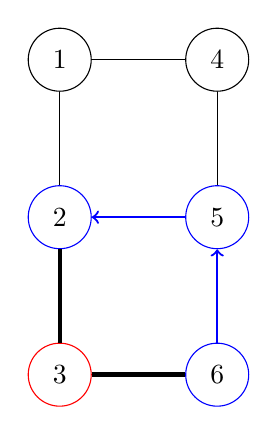
\begin{tikzpicture}[
  vertex/.style={draw,circle,minimum size=0.8cm},
  every node/.style={vertex},
  red_vertex/.style={draw=red},
  blue_vertex/.style={draw=blue},
  inx/.style={draw=black, ultra thick},
  red_edge/.style={draw=red, ultra thick},
  onc/.style={draw=blue, thick}
  ]
	\node (1) at (1,5) {1};
	\node[blue_vertex] (2) at (1,3) {2};
	\node[red_vertex] (3) at (1,1) {3};

	\node (4) at (3,5) {4};

	\node[blue_vertex] (5) at (3,3) {5};
	\node[blue_vertex] (6) at (3,1) {6};

	\draw (1) -- (2);
	\draw[inx] (2) -- (3);

	\draw (4) -- (5);
	\draw[onc,<-] (5) -- (6);

	\draw (1) -- (4);
	\draw[onc, <-] (2) -- (5);
	\draw[inx] (3) -- (6);
\end{tikzpicture}
 \\
 $X = \{ (2,3), (3,6) \}$
	\end{multicols}

\end{frame}

\begin{frame}
	\frametitle{Example}

    Colour one side of the future cut red and the other blue.
	\center
	\begin{multicols}{2}

		1. step (back from recursive call) \\
	\medskip
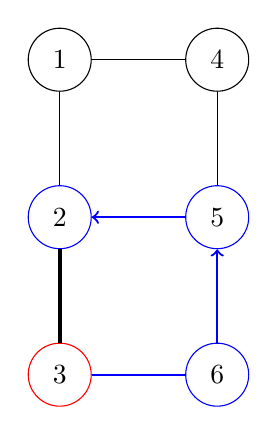
\begin{tikzpicture}[
  vertex/.style={draw,circle,minimum size=0.8cm},
  every node/.style={vertex},
  red_vertex/.style={draw=red},
  blue_vertex/.style={draw=blue},
  inx/.style={draw=black, ultra thick},
  red_edge/.style={draw=red, ultra thick},
  onc/.style={draw=blue, thick}
  ]
	\node (1) at (1,5) {1};
	\node[blue_vertex] (2) at (1,3) {2};
	\node[red_vertex] (3) at (1,1) {3};

	\node (4) at (3,5) {4};
	\node[blue_vertex] (5) at (3,3) {5};
	\node[blue_vertex] (6) at (3,1) {6};

	\draw (1) -- (2);
	\draw[inx] (2) -- (3);

	\draw (4) -- (5);
	\draw[onc, <-] (5) -- (6);

	\draw (1) -- (4);
	\draw[onc, <-] (2) -- (5);
	\draw[onc] (3) -- (6);
\end{tikzpicture}
 \\
 $X = \{ (2,3) \}$

1. step, 2. recursive call \\
	\medskip
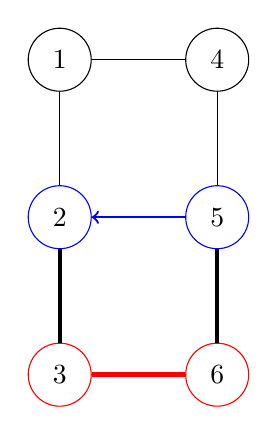
\begin{tikzpicture}[
  vertex/.style={draw,circle,minimum size=0.8cm},
  every node/.style={vertex},
  red_vertex/.style={draw=red},
  blue_vertex/.style={draw=blue},
  inx/.style={draw=black, ultra thick},
  red_edge/.style={draw=red, ultra thick},
  onc/.style={draw=blue, thick}
  ]
	\node (1) at (1,5) {1};
	\node[blue_vertex] (2) at (1,3) {2};
	\node[red_vertex] (3) at (1,1) {3};

	\node (4) at (3,5) {4};
	\node[blue_vertex] (5) at (3,3) {5};
	\node[red_vertex] (6) at (3,1) {6};

	\draw (1) -- (2);
	\draw[inx] (2) -- (3);

	\draw (4) -- (5);
	\draw[inx] (5) -- (6);

	\draw (1) -- (4);
	\draw[onc, <-] (2) -- (5);
	\draw[red_edge] (3) -- (6);
\end{tikzpicture}
 \\
 $X = \{ (2,3), (6,5) \}$
	\end{multicols}

\end{frame}
